\documentclass[11pt,letterpaper]{article}

% \usepackage{epstopdf}% To incorporate .eps illustrations using PDFLaTeX, etc.
% \usepackage[caption=false]{subfig}% Support for small, `sub' figures and tables
%\usepackage[nolists,tablesfirst]{endfloat}% To `separate' figures and tables from text if required
%\usepackage[doublespacing]{setspace}% To produce a `double spaced' document if required
%\setlength\parindent{24pt}% To increase paragraph indentation when line spacing is doubled

% \usepackage[longnamesfirst,sort]{natbib}% Citation support using natbib.sty
% \bibpunct[, ]{(}{)}{;}{a}{,}{,}% Citation support using natbib.sty
% \renewcommand\bibfont{\fontsize{10}{12}\selectfont}% To set the list of references in 10 point font using natbib.sty

\usepackage[natbibapa,nodoi]{apacite}% Citation support using apacite.sty. Commands using natbib.sty MUST be deactivated first!
\setlength\bibhang{12pt}% To set the indentation in the list of references using apacite.sty. Commands using natbib.sty MUST be deactivated first!
\renewcommand\bibliographytypesize{\fontsize{10}{12}\selectfont}% To set the list of references in 10 point font using apacite.sty. Commands using natbib.sty MUST be deactivated first!
\usepackage[english]{babel}
\addto{\captionsenglish}{%
    \renewcommand{\refname}{Referanslar}%
    \renewcommand{\contentsname}{Table of Contents}}

% \theoremstyle{plain}% Theorem-like structures provided by amsthm.sty
% \newtheorem{theorem}{Theorem}[section]
% \newtheorem{lemma}[theorem]{Lemma}
% \newtheorem{corollary}[theorem]{Corollary}
% \newtheorem{proposition}[theorem]{Proposition}

% \theoremstyle{definition}
% \newtheorem{definition}[theorem]{Definition}
% \newtheorem{example}[theorem]{Example}

% \theoremstyle{remark}
% \newtheorem{remark}{Remark}
% \newtheorem{notation}{Notation}

\usepackage[table,x11names,svgnames,dvipsnames]{xcolor}
\usepackage[export]{adjustbox}
% \usepackage{algorithm}
% \usepackage[noend]{algpseudocode}
\usepackage{amsmath,amssymb,amsfonts}
\usepackage[USenglish]{babel}
\usepackage{bigints}
\usepackage{bm}
\usepackage{booktabs}
\usepackage{cancel}
\usepackage[tableposition=above, font=normalsize]{caption}
% \usepackage{centernot}
% \usepackage{comment}
\usepackage{empheq}
\newcommand*\widefbox[1]{\fbox{\hspace{2em}#1\hspace{2em}}}
\usepackage{enumitem}
\usepackage{epsfig}
\usepackage{epstopdf}
% \epstopdfsetup{outdir=./figures//}
% \usepackage[letterpaper, top=1.0in, bottom=1.0in, left=1.0in, right=1.0in]{geometry}
\RequirePackage[OT1]{fontenc}
% \usepackage{fontspec}
\usepackage{graphics}
\usepackage{graphicx}
\graphicspath{{../figures/}}
% \usepackage{ifpdf}
% \usepackage{lastpage}
% \usepackage{leftidx}
\usepackage{lineno}
\usepackage{lipsum}
% \usepackage{mathrsfs}
\usepackage{mathtools}
\usepackage{multicol}
\usepackage{multirow}
\usepackage{nicefrac}
% \usepackage{nicematrix}
% \usepackage{pgfplots}
\usepackage{pifont}
% \usepackage{ragged2e}
% \usepackage{rotating}
% \usepackage{stmaryrd}
\usepackage{siunitx}
\usepackage{soul}
\usepackage[caption=false]{subfig}
\usepackage{tabularx}
\usepackage{threeparttable}
\usepackage{tikz}
% \usepackage{tkz-euclide}
% \usepackage{ctable}
% \usetikzlibrary{matrix, arrows}
\usetikzlibrary{shapes.geometric, arrows, decorations.markings, shapes.arrows}

\newcommand{\minitab}[2][l]{\begin{tabular}{#1}#2\end{tabular}}

%%%%%%% TODO NOTES 
\usepackage{todonotes}
\setlength{\marginparwidth}{1.3cm}
\setlength{\marginparsep}{0cm}
\newcommand{\ctodo}[1]{\todo[size=\tiny]{#1}}
\newcommand{\nnparam}{\theta}
\newcommand{\pinn}{\pi_{\nnparams}}

\usepackage{wrapfig}

\tikzstyle{startstop} = [rectangle, rounded corners, minimum width=1cm, minimum
height = 0.5cm, text centered, draw=black, fill=red!30]
\tikzstyle{io} = [trapezium, trapezium left angle=70, trapezium right angle=110,
minimum height=1cm, text width=3cm, text centered, draw=black, fill=blue!30]
\tikzstyle{process} = [rectangle, minimum width=2cm, minimum height=0.8cm, text
centered, text width=2cm, draw=black, fill=orange!30]
\tikzstyle{decision} = [diamond, aspect=1.25, minimum width=2cm, minimum height=0.5cm, 
text centered, text width=3cm, draw=black, fill=green!30]
\tikzstyle{arrow} = [thick, ->, >=stealth]




\makeatletter
\newcommand{\rmnum}[1]{\romannumeral #1}
\newcommand{\Rmnum}[1]{\expandafter\@slowromancap\romannumeral #1@}
\makeatother

\newcommand{\bmat}[1]{\begin{bmatrix}#1\end{bmatrix}}
\newcommand{\pmat}[1]{\begin{pmatrix}#1\end{pmatrix}}
\newcommand{\ubar}[1]{\text{\b{$#1$}}}
\newcommand{\norm}[2]{\|{#1}\|_{{}_{#2}}}
\newcommand{\abs}[1]{\left|{#1}\right|}
\newcommand{\mbf}[1]{\mathbf{#1}}
\newcommand{\mc}[1]{\mathcal{#1}}
\newcommand{\dd}{\operatorname{d}\!}
\newcommand{\muc}[2]{\multicolumn{#1}{c}{#2}}
\newcommand*\Eval[3]{\left.#1\right\rvert_{#2}^{#3}}
\newcommand{\inner}[1]{\left\langle#1\right\rangle}
\newcommand{\pd}[2]{\frac{\partial #1}{\partial #2}}
\newcommand{\pdd}[2]{\frac{\partial^2 #1}{\partial #2^2}}
\newcommand{\el}[2]{\frac{\dd}{\dd t}\pd{\mc{L}}{\dot{#1}} - \pd{\mc{L}}{#1} = #2}
\newcommand{\elk}[2]{\frac{\dd}{\dd t}\pd{\mc{L}}{\dot{#1}_k} - \pd{\mc{L}}{#1_k} = #2_k}
\newcommand{\vectornorm}[1]{\left|\left|#1\right|\right|}
\newcommand{\dom}[1]{\textrm{dom}\;#1}
\newcommand{\bx}{{\bf x}}
\newcommand{\bu}{{\bf u}}
\newcommand{\cmark}{\ding{51}}%
\newcommand{\xmark}{\ding{55}}%
\newcommand*{\vertbar}{\rule[-1ex]{0.5pt}{2.5ex}}
\newcommand*{\horzbar}{\rule[.5ex]{2.5ex}{0.5pt}}

\newcommand{\idapbc}{\textsc{IdaPbc}}
\newcommand{\electric}{{\textcolor{blue}{\hspace{-0.5mm}$\bm{E}$\;}}}
\newcommand{\magnetic}{{\textcolor{red}{\hspace{-0.5mm}$\bm{B}$\;}}}

% \theoremstyle{plain}
% \newtheorem{thm}{Theorem}[section]
\newtheorem{thm}{Theorem}
% \makeatletter
% \@addtoreset{thm}{section}
% \makeatother
% \newtheorem{cor}[thm]{Corollary}
\newtheorem{lem}{Lemma}
% \newtheorem{claim}[thm]{Claim}
% \newtheorem{axiom}[thm]{Axiom}
% \newtheorem{conj}[thm]{Conjecture}
% \newtheorem{fact}[thm]{Fact}
% \newtheorem{hypo}[thm]{Hypothesis}
% \newtheorem{assum}[thm]{Assumption}
\newtheorem{prop}{Proposition}
% \newtheorem{crit}[thm]{Criterion}
% \theoremstyle{definition}
\newtheorem{defn}[thm]{Definition}
% \newtheorem{exmp}[thm]{Example}
\newtheorem{rem}{Remark}
% \newtheorem{prin}[thm]{Principle}

\DeclareMathOperator{\Tr}{tr}
\newcommand\xdownarrow[1][2ex]{%
   \mathrel{\rotatebox{90}{$\xleftarrow{\rule{#1}{0pt}}$}}
}
\DeclareMathOperator{\End}{End}
\DeclareMathOperator{\Hom}{Hom}
\DeclareMathOperator{\id}{id}
\DeclareMathOperator{\vers}{vers}
\DeclareMathOperator{\trans}{Trans}
\DeclareMathOperator{\rot}{Rot}
\DeclareMathOperator{\rank}{rank}
\DeclareMathOperator{\sinc}{sinc}

\usepackage{hyperref}
\hypersetup{
    unicode=false,          % non-Latin characters in Acrobat’s bookmarks
    pdftoolbar=true,        % show Acrobat’s toolbar?
    pdfmenubar=true,        % show Acrobat’s menu?
    pdffitwindow=false,     % window fit to page when opened
    pdfstartview={FitH},    % fits the width of the page to the window
    pdftitle={Mischievous Sibling's Grid World},    % title
    pdfauthor={Aykut C. Satici}, % author
    % pdfsubject={Subject},   % subject of the document
    % pdfcreator={Creator},   % creator of the document
    % pdfproducer={Producer}, % producer of the document
    % pdfkeywords={keyword1, key2, key3}, % list of keywords
    pdfnewwindow=true,      % links in new PDF window
    colorlinks=true,       % false: boxed links; true: colored links
    linkcolor=blue!30!green,          % color of internal links (change box color with linkbordercolor)
    linkbordercolor=orange,
    citecolor=blue,        % color of links to bibliography
    citebordercolor=green,
    filecolor=magenta,      % color of file links
    urlcolor=cyan,           % color of external links
    urlbordercolor=blue,
}


\begin{document}

% \articletype{}% Specify the article type or omit as appropriate

% \title{\.{I}lgin\c{c} Bir Olas{\i}l{\i}k Sorusu}
\section*{
    \begin{center}
        Sonaj'in Zaman Yolculugu
    \end{center}
}

\begin{center}
    G\"{o}khan At{\i}n\c{c}\textsuperscript{} ve Aykut C. Sat{\i}c{\i}\textsuperscript{} \\[0ex]
    % 1 Temmuz 2021
\end{center}


  
\vspace{-1mm}
\section{Problem Statement}

\definecolor{blue538}{HTML}{30a2da}
\definecolor{red538}{HTML}{fc4f30}
\definecolor{yellow538}{HTML}{e5ae38}
\definecolor{green538}{HTML}{6d904f}
\definecolor{gray538}{HTML}{8b8b8b}
%
% \begin{wrapfigure}{r}{0.4\textwidth} %this figure will be at the right
%     \vspace{-5mm}
%     \centering
%     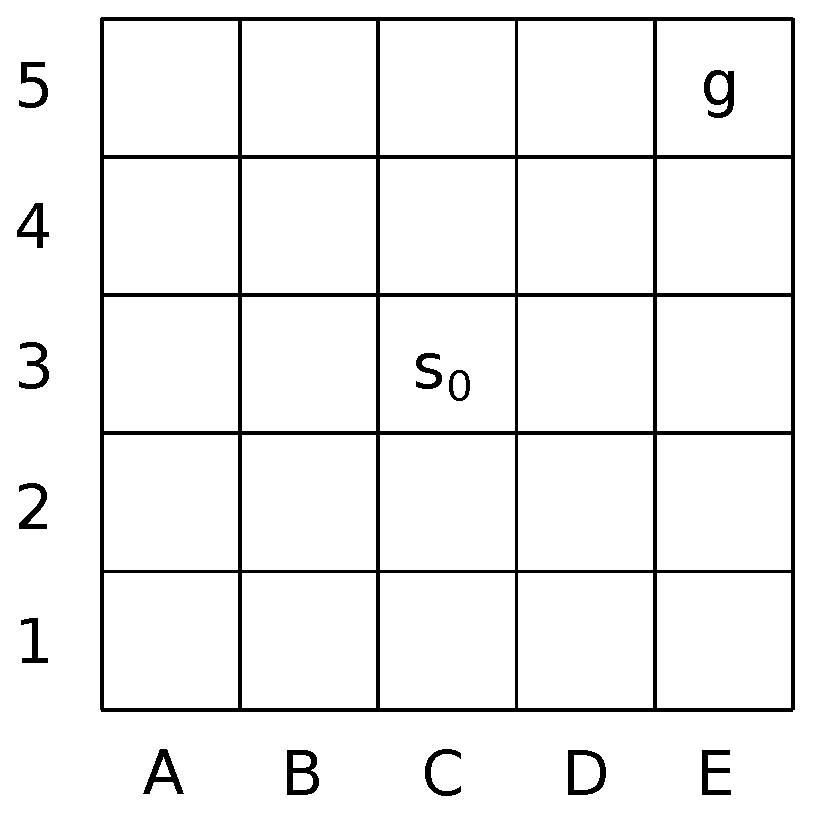
\includegraphics[width=0.25\textwidth]{./figures/drawing.eps}
%     \caption{Problemin \c{s}emati\u{g}i}
%     \label{fig:schematic}
%     \vspace{-5mm}
% \end{wrapfigure}
%
\begin{minipage}{0.5\textwidth}
    Points $P$ and $Q$ are randomly sampled from a uniform distribution on two
    sides of a unit square. Let $d$ be the random variable that denotes the
    length of the chord $\abs{PQ}$ (see the figure). What is the probability
    that $d \geq 1$?
\end{minipage}
\begin{minipage}{0.5\textwidth}
    \begin{center}
\begin{tikzpicture}[scale=2]
    % \draw (0, 0) -- (1.5, 0);
    % \draw (0, 0) -- (0, 1.5);
    %
    % \draw[ultra thin, gray, step=.1cm] (0, 0) grid (1.5, 1.5);
    %
    % \draw[ultra thick, blue538] (0, 0) rectangle (1, 1);
    \draw[ultra thick] (0, 0) rectangle (1, 1);
    %
    \foreach \x/\xtext in {0, 1}
    \draw (\x cm, 1pt) -- (\x cm,-1pt) node[anchor=north] {$\xtext$};
    \foreach \y/\ytext in {0, 1}
    \draw (1pt,\y cm) -- (-1pt,\y cm) node[anchor=east] {$\ytext$};
    %
    \node[above] (P) at (0.6, 1) {$P$};
    \node[right] (Q) at (1, 0.2) {$Q$};
    \draw (0.6, 1) -- (1, 0.2);
    \draw[fill=black] (0.6, 1) circle (.03cm);
    \draw[fill=black] (1, 0.2) circle (.03cm);
\end{tikzpicture}
\end{center}
\end{minipage}

\section{Problem Solution}
\label{sec:solution}

Shown in Figure~\ref{fig:unfolded}, we show the regular pyramid of
Figure~\ref{fig:problem} unfolded onto the plane in such a manner that the edge
$OQ$ remains glued, while the edges $OR$, $OS$, and $OP$ are unglued. An
arbitrary piecewise straight path $\gamma$ from the vertex $P$ to the midpoint
$T$ is then depicted as the green curve on this figure. The continuous portions,
$PU$ and $UT$, of this path have lengths $\ell_1$ and $\ell_2$, respectively.

The line $PR$ that connects the vertices $P$ and $R$ is orthogonal to the edge
$OQ$ since the triangle $\triangle POQ$ is equilateral. Let the signed distance
from the intersection $M$ of $PR$ with $OQ$ to the intersection $U$ of our path
$\gamma$ and $OQ$ be given by $x$. In the following, we express the total length
$\ell_1 + \ell_2$ of our curve $\gamma$ as a function of this distance $x$ and
minimize it to arrive at the answer.

\begin{figure}[h]
  \centering
  \includegraphics[trim={0 0 0
  0cm},clip,width=0.5\textwidth]{./figures/pyramid-unfolded.pdf}
  \vspace{-8mm}
  \caption{The unfolded regular pyramid.}
  \label{fig:unfolded}
\end{figure}

Since $PM \perp OM$, Pythagoras's theorem yields $\abs{PM} = \sqrt{3}\ell$. By
the same token, $\triangle PMU$ is a right triangle, yielding 
%
\begin{equation}
    \ell_1(x) = \sqrt{x^2 + 3\ell^2}. 
    \label{eq:ell1}
\end{equation}    
%
The perpendicular $TM^\prime$ to $PR$ is parallel to $OQ$ so by the similarity
of the triangles $\triangle OMR$ and $\triangle TM^\prime R$, and the fact that
$\abs{OM} = \ell$, we deduce that $\abs{TM^\prime} = \nicefrac{\ell}{2}$ and
$\abs{MM^\prime} = \nicefrac{\sqrt{3}\ell}{2}$. Using these lengths, along with
$x$, as the side lenghts of the orange right triangle $\triangle T\tilde{M}M$ in
Figure~\ref{fig:unfolded}, we obtain 
%
\begin{equation}
  \ell_2(x) = \sqrt{\ell^2 + \ell x + x^2}.
  \label{eq:ell2}
\end{equation}

The solution that we seek minimizes $\ell_1(x) + \ell_2(x)$. Therefore, we
differentiate this function and set it equal to zero to obtain \[
\frac{2x}{\sqrt{3\ell^2 + x^2}} + \frac{\ell+2x}{\sqrt{\ell^2 + \ell x + x^2}} =
0. \] The solution to this equation is $x^\star = -\nicefrac{\ell}{3}$ as a
simple substitution will show. Plugging this solution into
equations~\eqref{eq:ell1} and~\eqref{eq:ell2} yields \[ \ell_1^\star =
\ell_1(x^\star) = \frac{2\sqrt{7}}{3}\ell, \qquad \ell_2^\star =
\ell_2(x^\star)= \frac{\sqrt{7}}{3}\ell. \] Summing these two optimal values
gives the shortest distance between points $P$ and $T$ on the regular square
pyramid as \[ \ell_1(x^\star) + \ell_2(x^\star) = \sqrt{7}\ell. \]

\begin{lemma}{\textbf{Lemma 1.}}
  The (green) path that yields the shortest distance $\sqrt{7}\ell$ is a
  straight line.
\end{lemma}

\begin{proof}
    Perhaps the easiest way to show this is to use the law of cosines to show
    that the edge $PT$ of the triangle $\triangle POT$ has length equal to
    $\sqrt{7}\ell$ so that our solution for the green path coincides with the
    dash-dotted red line on Figure~\ref{fig:unfolded}.

    \begin{align*}
        \abs{PT}_{\text{red}}^2 &= (2\ell)^2 + \ell^2 - 2 \cdot 2\ell \cdot \ell
        \cos{120^\circ} = 7\ell^2
    \end{align}
\end{proof}

\section{Say{\i}sal \c{C}\"{o}z\"{u}m}
\label{sec:numerical}

Bolum~\ref{sec:solution}'de acikladigimiz yontemi uygulamak icin
Julia~\citep{bezanson2017julia} programlama dilinde yazilmis olan
JuMP~\citep{DunningHuchetteLubin2017} paketini ve Mosek~\citep{mosek}
cozumleyicisini kullandik.

\begin{table}[h]
\caption{Eniyileme sonuclari}
\label{tab:optimization_results}
\centering
\begin{tabular}{l|cccccc}
   $N$ & $0$ & $1-3$ & $4$ & $5$ & $6$ & $7-10$ \\ \hline
   $T$ & $0$ & Olursuz & 33 & Olursuz & 55 & Olursuz \\
   $\alpha + \beta + \gamma$ & $36$ & Olursuz & $82.625$ & Olursuz & $104$ & Olursuz 
\end{tabular}
\end{table}

Sonaj'in zamanda gorebilecegi en ileri tarih, yani eniyileme programimizin $T$
olarak hesapladigi deger $N=6$ icin elde edilmis. Bu durumda bize sorunun
sordugu niceligin degeri de \[ \alpha + \beta + \gamma = 104 \] olarak bulunmus.
Merakimizi gidermek icin $N=6$ icin Sonaj'in izledigi yorungeyi de asagida
kaydedelim:

\begin{table}[h]
    \caption{Sonaj'in en iyi yorungesi}
    \label{tab:trajectory}
    \centering
    \begin{tabular}{l|ccc}
       $k$ & Yas & Secium miktari & Zaman (Yil) \\ \hline
       $1$ & $15$ & 21 & $0$ \\
       $2$ & $15$ & 20 & $33$ \\
       $3$ & $26$ & 10 & $44$ \\
       $4$ & $37$ & 5 & $55$ \\
       $5$ & $37$ & 4 & $22$ \\
       $6$ & $48$ & 2 & $33$ \\
       $7$ & $48$ & 1 & $0$
    \end{tabular}
\end{table}

\bibliographystyle{apacite}
\bibliography{bib/main}

\end{document}
